\begin{frame} [fragile]
	\frametitle{RAD - $R$adiation $A$ssessment $D$etector}
	\begin{columns}
  		\begin{column}{0.50\textwidth}
			Il 31 maggio 2013, gli scienziati della NASA hanno riportato i risultati ottenuti durante la crociera e hanno affermato che \colorbox{yellow}{il valore della dose equivalente} per il viaggio di sola andata e senza sosta ($t_{tot}$ $\sim$ $1$ anno) con i sistemi di propulsione e di schermatura attuali risulta essere  \colorbox{yellow}{0.66 $\pm$ 0.12 Sivert}. 
			\newline

			L'esposizione a 1 $Sv$ aumenta il rischio di morte per cancro di $\sim$ $5$$\%$ $\Longrightarrow$ \textcolor{red}{Grande rischio} per la salute \newline
			\textcolor{red}{per qualsiasi missione} umana su Marte. 
		\end{column}
    \begin{column}{0.50\textwidth}
 		\newline
			\begin{figure}
	  		\centering
				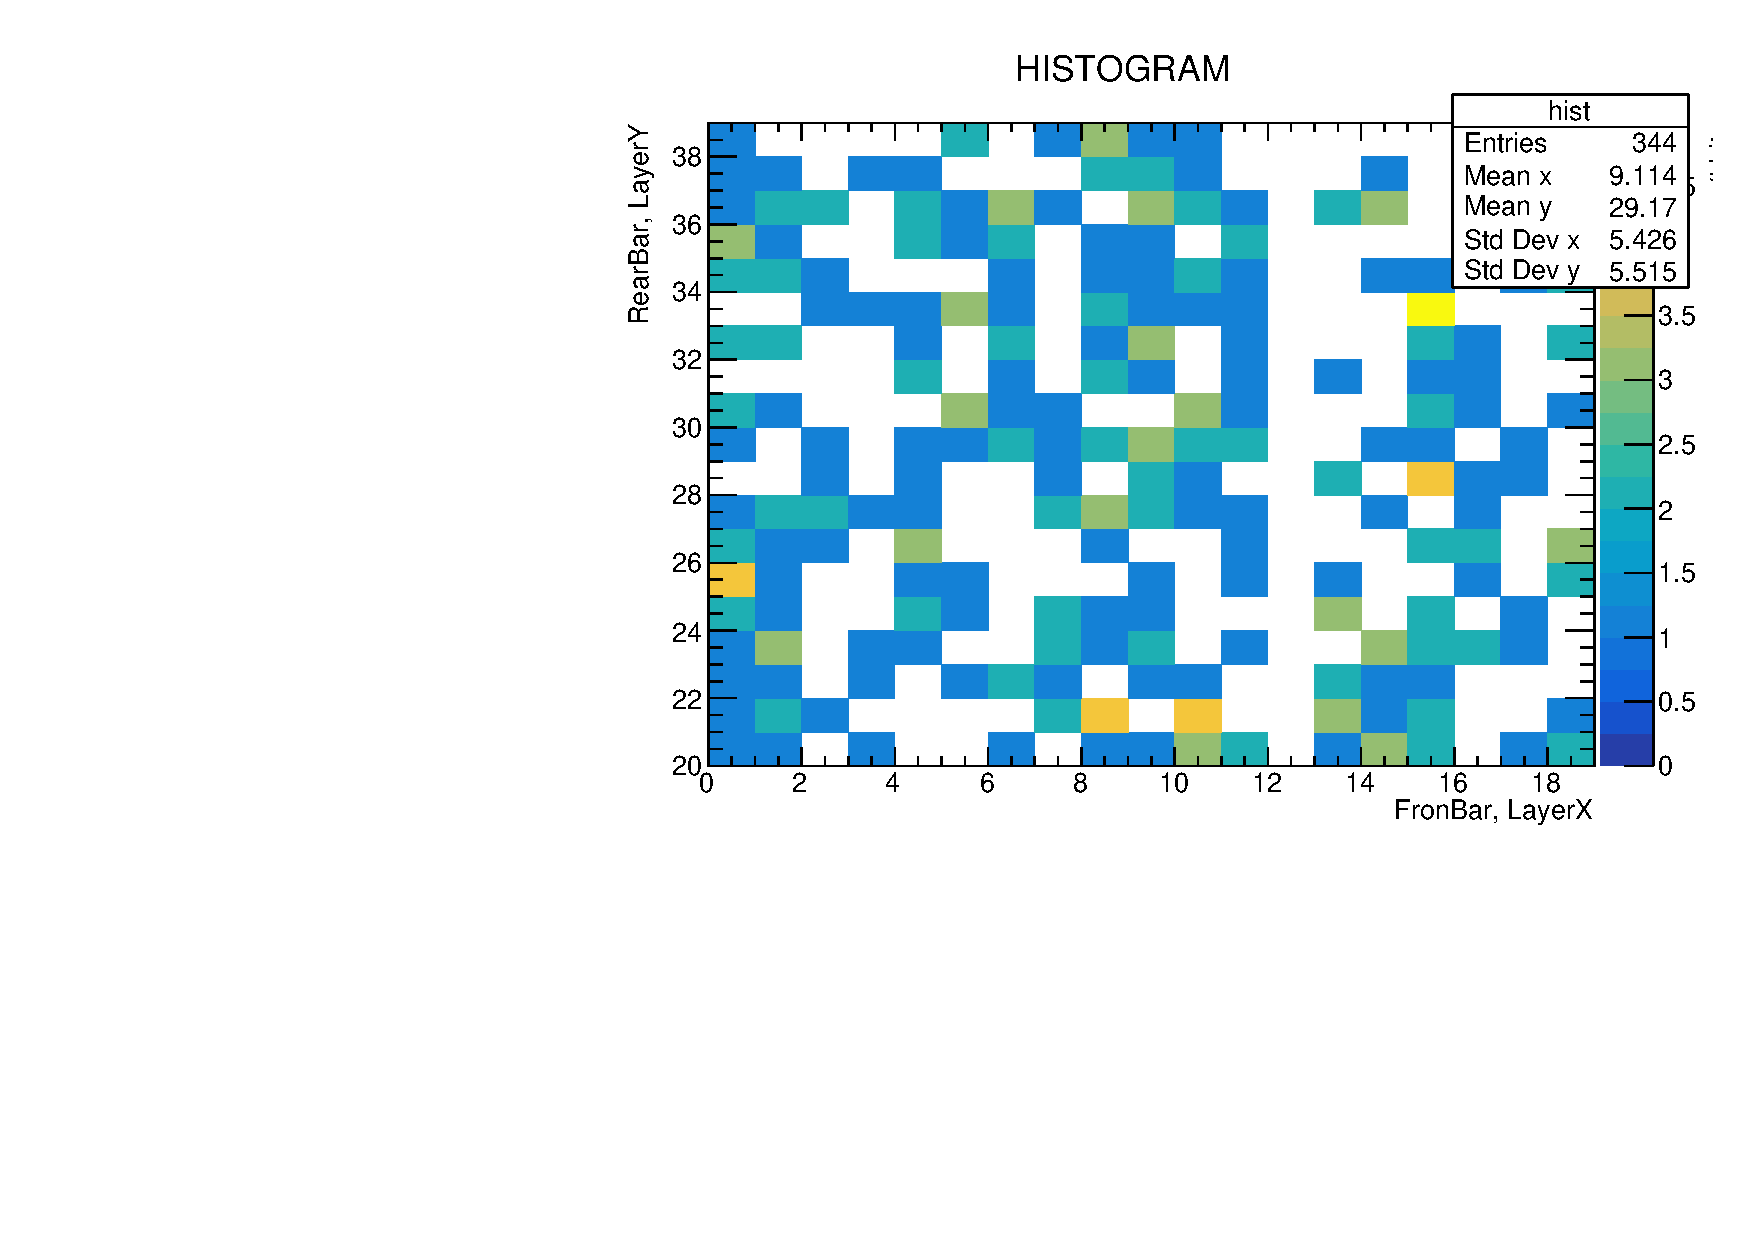
\includegraphics[scale=0.20]{figures/0.20.pdf}
				%\caption{Spettri energetici di diversi ioni nei GCR \cite{saggiatore}}
				\end{figure}
			\begin{block}{}
				RAD: calorimetro $CsI$ per particelle cariche e raggi $\gamma$
			\end{block}
    \end{column}
\end{columns}
\end{frame}